This section will present techniques that improve the accuracy of the detector but are not part of the architecture in itself. Those techniques applies during training but not during inference, so they do not increase the inference computing cost.

\section{Data Augmentations}
Deep Learning is known for requiring vast amount of data in order to train it properly and avoid \gls{overfit}\cite{shorten2019}. However, most domains which requires Deep Learning do not possess the amount of data that is required and this issue is particularly true here: see section~\ref{diffDataset}.  

Data Augmentation is a solution to this issue and tries to enhance both the size and quality of the dataset so that a more robust model can be trained. It makes the examples "harder", by adding variability to the dataset. This is done by modifying the image in various way, with color modification or geometric transformations. We will describe here the augmentations that are used in our model.

\subsection{Image Modification}
An issue seen in \gls{lidar} is the fact that object are often occluded, fragmented and do not appear with the same clarity as examples seen in satellite imagery. This means that we need to construct and train a network that is robust to changes in context and occlusion. Fortunately, research has been focussed in constructing better data augmentation techniques that attempt to solve those issues. Those techniques "mixes" different images from the dataset, covering parts of one another to make it harder for the network to correctly infer. CutMix\cite{cutMix} is one of those techniques. Mosaic, introduced by Bochkovsky, Wang and Liao in the YOLOv4 paper\cite{yolov4} creates a new images out of 4, by creating a "mosaic" of sort, where the 4 images can take varying portions of the new image. 

\subsection{Regularization and Normalization}
Regularization reduce the complexity of a network and prevents overfitting. This is usually done by "dropping" random connections in a network, and training without those connections, a technique known as DropOut\cite{dropOut}. DropBlock\cite{dropBlock} relies on a similar method, but is more suitable for convolutional networks. DropBlock works by first choosing random seed points in a mask, and dropping a continuous region around those points. This is more effective than removing purely random activation as close activations contain closely related information.

\begin{figure}[H]
	\begin{subfigure}[t]{.3\textwidth}
  \centering
  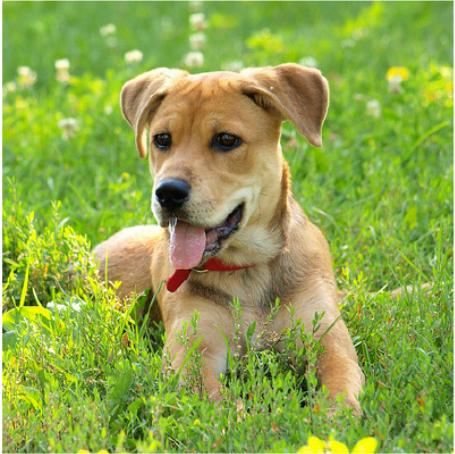
\includegraphics[width=.8\linewidth]{dogDropBlock}
  \caption{Base image}
  \label{fig:dropBlockA}
\end{subfigure}
	\begin{subfigure}[t]{.3\textwidth}
  \centering
  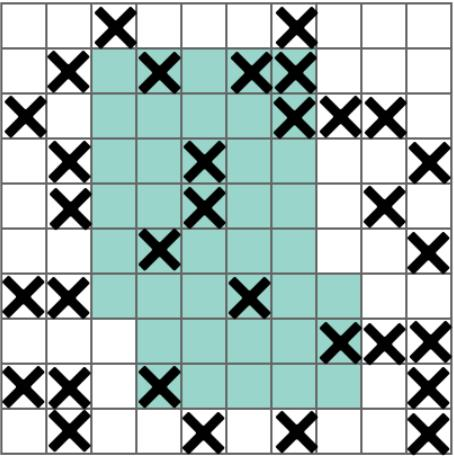
\includegraphics[width=.8\linewidth]{randomDrop}  
  \caption{Random Drop in activations}
  \label{fig:dropBlockB}
\end{subfigure}
	\begin{subfigure}[t]{.3\textwidth}
  \centering
  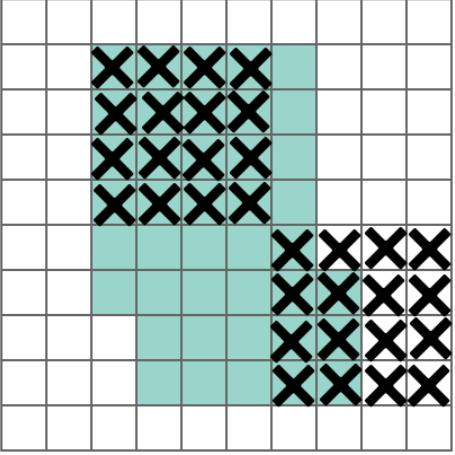
\includegraphics[width=.8\linewidth]{dropBlock}  
  \caption{DropBlock}
  \label{fig:dropBlockC}
\end{subfigure}
	\caption[Regularisation by dropping: random drops \textit{v.s.} DropBlock]{Regularisation by dropping: random drops \textit{v.s.} DropBlock\\The blue regions represents neurons that contains semantic information on the base image. (b) shows the effect of removing activations at random, which is not effective as neurons close to each other contains closely related semantic information. (c) shows the DropBlock method, which have a better chance of entirely removing important semantic information on the base image, such as the head or the feet of the dog, forcing the remaining neurons to learn useful features}
\label{fig:dropBlock}
\end{figure}

Label smoothing~\cite{labelSmooth} convert hard labels, like one hot labeling into soft labels. This works by introducing a noise distribution in the labeling of the data, and converting the original label in relation to this noise distribution. \textbf{However, this label smoothing requires a rewriting of the loss system.}

\section{Self Adversarial Training}
In the YOLOv4\cite{yolov4} paper, the author mention the use of \textbf{self adversarial training}. In this training regime, the network first tries to alter the original image instead of its weights. This is an adversarial attack on itself, modifying the original image to fool itself into a wrong inference. Then, the network is trained to detect an object on this modified image in the normal way.

\subsection{Modifications on the original dataset}
In total, 4 different datasets where used. Those dataset kept the general philosophy, explained in section ~\ref{dataset}, where an object is selected to be the center of cropped image, with randomised jitter added.

\begin{itemize}
	\item \textbf{Version 1}: The first version of this dataset used $1000 \times 1000$ pixels images, where object seen in another example could be reused
	\item  \textbf{Version 2}: The second version also used $1000 \times 1000$ pixels images, but object seen in another example could not be reused. The aim of this modification was to improve the variability of images. This greatly reduced the raw number of images in the dataset, from about 3000 to slightly more than a thousand, which in turn gave way to a loss in performance.
	\item \textbf{Version 3}: The third version used $500 \times 500$ pixels images, where object seen in another example could be reused. Smaller images meant that inference could be done without downscaling. 
	\item  \textbf{Version 4}: The final version used $1000 \times 1000$ pixels images, where object seen in another example could be reused. In addition to the images centered a particular object, a further 1000 images centered around random coordinates in random base images were added. This meant that the dataset now had images that could contain no objects. This gave the best results. 
\end{itemize}


